\section{Propagation geometry and calibration cost}
\label{supp:note5}

\subsection*{Ray-traced channels and the unit of comparison}
The O1\_60 street and ASU Campus 1 scenes provide two propagation geometries from the DeepMIMO collection~\cite{deepmimo}. Each uses base station 1 and 64 disjoint guarded test tiles. The source carrier frequencies are 60 and 3.5 GHz. The tile widths are approximately 1.20 and 12 m, respectively. Thus the comparison combines carrier, propagation geometry and spatial sampling. The same frozen tile supplies nested sets of \(K=16,32,64\) users. Its \(S=K/2\) tones are evenly spaced crops of the original 64-tone, 20-MHz channel. The block scaling used in the archived 10-dB run is applied before computing rates, so the diagnostic follows exactly the normalization of the reported schedule.

Let \(h_{is}\) denote the resulting whitened channel and \(u_{is}=h_{is}/\|h_{is}\|\). On each tone we form the Gram matrix \(Q_s\), whose entries are \(u_{is}^{H}u_{js}\). The two spatial summaries are
\begin{align}
r_{\rm tile}&=\frac{1}{S{K\choose2}}\sum_s\sum_{i<j}|u_{is}^{H}u_{js}|^2,\\
d_{\rm tile}&=\frac1S\sum_s\exp\left(-\sum_\ell t_{\ell s}\ln t_{\ell s}\right),
\qquad t_{\ell s}=\frac{\lambda_\ell(Q_s)}{\operatorname{tr}Q_s},
\end{align}
with \(0\ln0=0\). The effective rank is one for perfectly parallel channels. Its upper bound is the smaller of \(K\) and the 16 receive dimensions. The implementation computes the equal nonzero eigenvalues of the antenna Gram matrix to avoid an unnecessarily large eigendecomposition.

To separate partner choice from power adaptation, fix every user's power at \(p=0.10\) W. For a candidate partner \(j\), the recomputed linear-MMSE rate is
\begin{equation}
R_{i|j,s}=\log_2\left[1+p\|h_{is}\|^2
\left(1-\frac{p\|h_{js}\|^2|u_{is}^{H}u_{js}|^2}
{1+p\|h_{js}\|^2}\right)\right].
\end{equation}
For each user and tone, take the difference between the 90th and 10th percentiles over its \(K-1\) possible partners, using linear sample-quantile interpolation. Average these differences over users and tones to obtain the tile's partner-rate span. Every candidate comparison satisfies the same individual power rails and total budget.

The path counts and direct-path flags come from the original base-station ray records. For each tile, the path statistic is the median count over its selected users. The scene summary is the median of these 64 tile statistics, which can be nonintegral. The LoS statistic instead counts flagged user links over the whole cohort. The channel construction retains at most 25 rays per link. In this comparison, the 32- and 64-user geometry calculations reproduce the previously archived diagnostics. The 16-user calculation uses the same channel digests, original ray-file hashes and nested user ordering, rather than an independent resampling.

\begin{table}[htbp]
\centering
\caption{Ray geometry and certified-gap components at nominal 10 dB. Each row represents 64 guarded tiles. Geometry and rate entries are medians of tile-level values. LoS entries are counts of flagged user links. All rates, gaps and \(T_j\) entries are in bit/s/Hz. Component medians are computed separately and need not sum to the median gap.}
\label{supp:table6}
\small
\begin{tabular}{llrrrrr}
\hline
Scene & \(K\) & Overlap & Effective rank & Paths & LoS links & Partner span\\
\hline
O1 &16&0.9941&1.0199&3.25&1024/1024&1.0536\\
O1 &32&0.9936&1.0218&3.00&2048/2048&1.3234\\
O1 &64&0.9936&1.0230&3.00&4096/4096&1.4779\\
ASU &16&0.4790&2.4907&10.00&116/1024&1.8934\\
ASU &32&0.4649&2.6004&10.00&233/2048&1.9684\\
ASU &64&0.4578&2.6444&10.00&479/4096&2.0964\\
\hline
\end{tabular}

\medskip
\begin{tabular}{llrrrrr}
\hline
Scene & \(K\) & Gap & \(T_1\) & \(T_2\) & \(T_3\) & \(T_4\)\\
\hline
O1 &16&1.1097&0.0000&0.0036&\(6.8793\times10^{-7}\)&1.0929\\
O1 &32&1.1196&0.0004&0.0052&\(6.8793\times10^{-7}\)&1.1133\\
O1 &64&1.0956&0.0002&0.0129&\(6.8793\times10^{-7}\)&1.0713\\
ASU &16&0.0875&0.0232&0.0343&\(6.8793\times10^{-7}\)&0.0093\\
ASU &32&0.1016&0.0199&0.0479&\(6.8793\times10^{-7}\)&0.0074\\
ASU &64&0.0950&0.0137&0.0564&\(6.8793\times10^{-7}\)&0.0053\\
\hline
\end{tabular}
\end{table}

\begin{table}[htbp]\centering\small
\setlength{\tabcolsep}{4pt}
\caption{O1 enclosure width, partition depth and small continuous references at 10 dB. Each experiment uses the same 64 guarded tiles.}\label{supp:refinement}
\begin{tabular}{lllll}\toprule
Entries refined & Entries changed & Scheduled in shortlist & Median $G$ & Median $T_4$\\
\midrule
32 & 0 & 0/2/5 & 1.119582 & 1.113253\\
128 & 0 & 0/3/8 & 1.119582 & 1.113253\\
512 & 0 & 2/7/14 & 1.119582 & 1.113253\\
7936 & 0 & 16/16/16 & 1.119582 & 1.113253\\
\bottomrule\end{tabular}
\par\medskip\begin{minipage}{\linewidth}\small
\par\smallskip\noindent\begin{tabular}{rrrr}\toprule Children per selected entry & Median changed entries & Median $G$ & Median $T_4$\\\midrule
16 & 0 & 1.119582 & 1.113253\\
64 & 0 & 1.118334 & 1.080005\\
256 & 16 & 1.117494 & 0.867040\\
\bottomrule\end{tabular}\par\smallskip
\noindent\begin{tabular}{rlrrrr}\toprule $K$ & Statistic & Gap & Ceiling slack & Action loss & Reference width\\\midrule
2 & Mean & 1.173983 & [1.03877, 1.03877] & [0.13522, 0.13522] & 1.37e-15\\
2 & Median & 1.340835 & [1.18529, 1.18529] & [0.09974, 0.09974] & 1.33e-15\\
4 & Mean & 1.056186 & [0.90425, 0.90425] & [0.15193, 0.15193] & 9.55e-07\\
4 & Median & 1.118458 & [0.94817, 0.94817] & [0.16614, 0.16614] & 9.9e-07\\
\bottomrule\end{tabular}\par\smallskip
The width sweep partitions every chosen rectangle into 16 children. No upper-table tick changes on any tile at any budget: the child mixed signal/interference bounds remain above the parent tangent/box bound. The action has 16 scheduled entries; the shortlist column gives their minimum/median/maximum counts in the refined set. The depth sweep instead refines these 16 entries into 16, 64 or 256 children while keeping the original action, powers and tone/power prices fixed. Matching upper witnesses and the four-term identity are rebuilt and checked. Small references use the nested first two/four users of all 64 O1 tiles with the original channel normalization. Two-user roots are exact to their reported outward numerical enclosures; four-user complete labelled enumeration uses validated continuous Taylor/box bounds to $10^{-6}$ bit/s/Hz. All rates are bit/s/Hz; different $K$ have different feasible problems.
\end{minipage}
\end{table}


\subsection*{Reading the decomposition alongside the geometry}
The integer power scale is \(P_T=20\cdot2^{20}\). Projection rounds each scaled excess power down by less than one tick, leaving a small deterministic unused-power charge when the sum budget is active; the repeated median \(T_3=6.8793\times10^{-7}\) bit/s/Hz reflects these power ticks. The four normalized terms retain the definitions of Supplementary Note~2. \(T_1\) measures slack between the certified matching upper and the chosen partners' priced scores, \(T_2\) measures the cost of assigning distinct tones to those partners, \(T_3\) prices unused power, and \(T_4\) compares local continuous-power upper scores with the achieved-action lower rate. The sum is checked against the stored gap for all 384 tile--size records. At each size \(T_4\) has the largest component median on O1, while \(T_2\) has the largest component median on ASU. In particular, at 32 users ASU's \(T_2=0.0479\) exceeds its \(T_1=0.0199\), \(T_4=0.0074\) and \(T_3=6.8793\times10^{-7}\).

O1's nearly unit overlap and effective rank close to one indicate little spatial discrimination between users. Direct and reflected rays can reinforce nearly aligned array responses even when several physical paths are present. This helps interpret the large local rate interval on O1. The fixed-power partner span is nevertheless smaller there than on ASU at all three sizes. A large \(T_4\) therefore quantifies looseness between a local upper calculation and a particular achieved lower rate, rather than measuring sensitivity of user rate to partner choice. Figure~\ref{supp:fig5} displays the distributions underlying the summaries.

\begin{figure}[htbp]
\centering
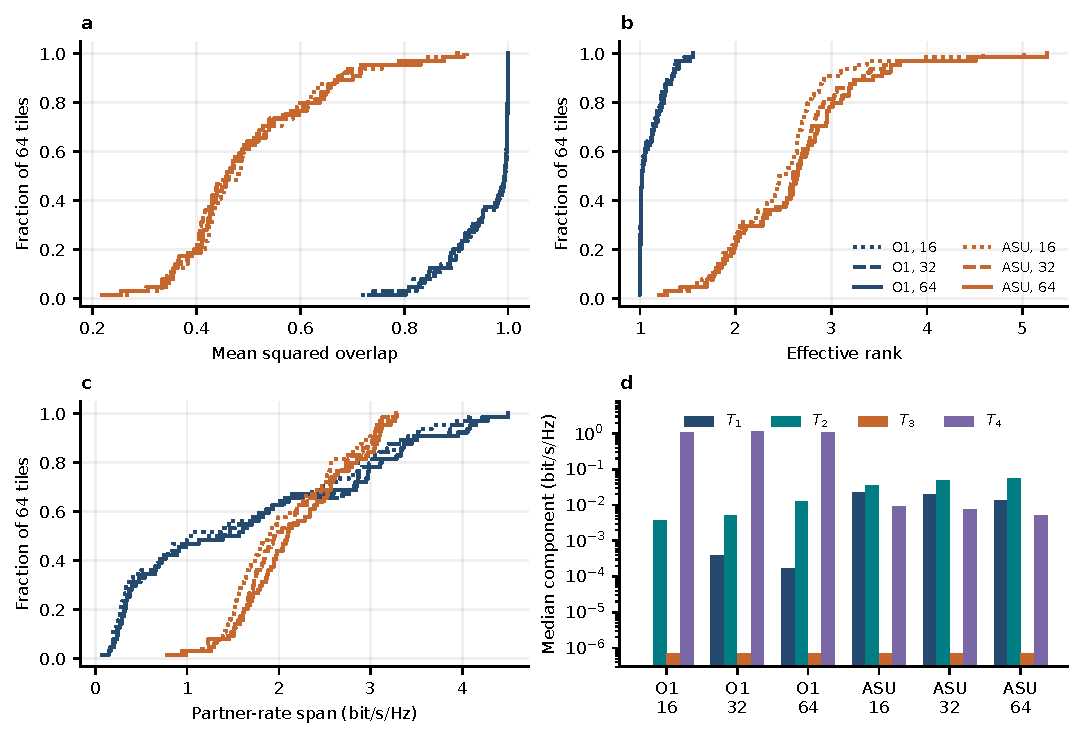
\includegraphics[width=\textwidth]{supplementary/figures/sfig5.pdf}
\caption{Propagation geometry and the four-term decomposition. \textbf{a--c}, Empirical cumulative distributions across 64 guarded tiles per scene and size. Colour identifies the scene, and dotted, dashed and solid curves identify 16, 32 and 64 users. The overlap, effective rank and fixed-power partner span are calculated as defined in this note. \textbf{d}, Separately calculated medians of the four normalized gap components on a logarithmic scale. A zero \(T_1\) median for 16-user O1 has no positive height on this scale. No uncertainty bars are plotted.}
\label{supp:fig5}
\end{figure}

\subsection*{Charging for pilots over a stationary horizon}
The net-gain experiment evaluates two fixed feasible actions on the same least-squares channel estimate, the zero-price, equal-power-initialized matching control with feasible power refinement \(c\) and a learned-initialized action \(w\). The rate intervals \([l_c,u_c]\) and \([l_w,u_w]\) use the stored powers, pairs and receive filters. Four calibration events, two per policy, share a total error probability of 0.05. Each uses rank \(\lceil257(1-0.0125)\rceil=254\) among 256 independent calibration blocks.

A block contains 256 symbols with 32 routine pilot symbols. Charging the warm action for \(M\) additional 32-symbol reference blocks over \(N_{\rm blk}\) stationary blocks gives
\begin{equation}
\eta_c=1-\frac{32}{256},\qquad
\eta_w=\max\left(0,\eta_c-\frac{32M}{256N_{\rm blk}}\right),
\end{equation}
and the budget is affordable if \(32M+32N_{\rm blk}\leq256N_{\rm blk}\). The net-rate interval is
\begin{equation}
[\eta_w l_w-\eta_c u_c,\ \eta_w u_w-\eta_c l_c].
\end{equation}
A positive outcome requires affordability and a lower endpoint above \(10^{-5}\) bit/s/Hz. A negative outcome requires affordability and an upper endpoint below \(-10^{-5}\). The remaining affordable cases are indeterminate. The evaluated horizons are \(1,4,16,64,256,1024\), and extra pilot-block counts are \(0,16,64,256,1024\). Each of the four channel/energy arms contains 128 held-out topologies. Holding the rates fixed makes the \(M=0\) fraction independent of \(N_{\rm blk}\). Transporting this calculation to a changing future channel sequence would require uncertainty calibration over that sequence.

\begin{table}[htbp]\centering\small
\setlength{\tabcolsep}{4pt}
\caption{Stationary net-rate outcomes and exact two-sided 95\% binomial intervals over independent simulated topologies. Each comparison includes 128 test topologies. The zero-additional-pilot fraction is the same at all evaluated horizons. Both actions use the same least-squares observation; the comparator includes its feasible power refinement.}\label{supp:table7}
\begin{tabular}{lllll}\toprule
Channel / pilots & Extra blocks & $N_{\rm blk}$ & Positive gain & 95\% interval (\%)\\
\midrule
CDL-C fixed & 0 & 1 & 0/128 & [0.0, 2.8]\\
CDL-C fixed & 16 & 256 & 0/128 & [0.0, 2.8]\\
CDL-C fixed & 16 & 1024 & 0/128 & [0.0, 2.8]\\
CDL-C scaled & 0 & 1 & 28/128 & [15.1, 30.0]\\
CDL-C scaled & 16 & 256 & 0/128 & [0.0, 2.8]\\
CDL-C scaled & 16 & 1024 & 0/128 & [0.0, 2.8]\\
UMa fixed & 0 & 1 & 12/128 & [4.9, 15.8]\\
UMa fixed & 16 & 256 & 0/128 & [0.0, 2.8]\\
UMa fixed & 16 & 1024 & 5/128 & [1.3, 8.9]\\
UMa scaled & 0 & 1 & 111/128 & [79.6, 92.1]\\
UMa scaled & 16 & 256 & 10/128 & [3.8, 13.9]\\
UMa scaled & 16 & 1024 & 74/128 & [48.8, 66.5]\\
\bottomrule\end{tabular}
\end{table}



\begin{figure}[htbp]\centering
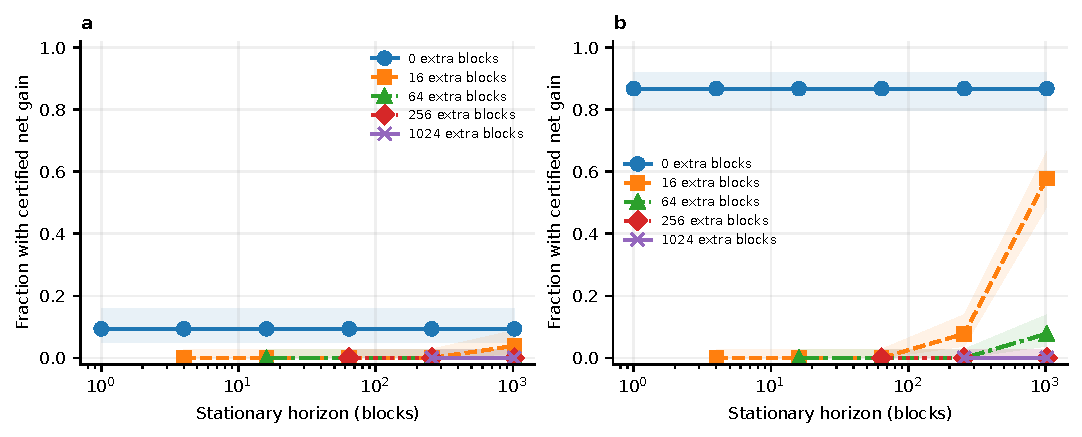
\includegraphics[width=\textwidth]{supplementary/figures/sfig6.pdf}
\caption{Stationary net-rate accounting. Fractions with a certified positive net advantage are shown against the number of stationary blocks for fixed and scaled pilot energy. Curves identify additional pilot-block charges. Only affordable points are drawn. Shaded bands are exact two-sided 95\% binomial intervals over 128 independent simulated topologies; they do not describe uncertainty about an unobserved future time series.}\label{supp:fig6}
\end{figure}
